

\section{integer overflow}
\begin{frame}{bounds-checking?}
    \begin{itemize}
    \item so far: mistake is no bounds checking
    \item run input function without telling it how much space
    \vspace{.5cm}
    \item so, we avoid this by checking sizes, right?
    \item common problem: bugs in size checking code
    \item integer overflow (or underflow)
    \end{itemize}
\end{frame}



\begin{frame}[fragile,label=intOverflowEx]{integer overflow example (1)}
\lstset{
    language=C,
    morekeywords=item,
    style=smaller,
    moredelim={**[is][\btHL<2|handout:0>]{~2~}{~end~}},
}
\begin{tikzpicture}
\node[anchor=north east] (code) at (-1,0) {
\begin{lstlisting}
item *load_items(int len) {
  int total_size = ~2~len * sizeof(item);~end~
  if (total_size >= LIMIT) {
    return NULL;
  }
  item *items = malloc(total_size);
  for (int i = 0; i < len; ++i) {
    int failed = read_item(&items[i]);
    if (failed) {
      free(items);
      return NULL;
    }
  }
  return items;
}
\end{lstlisting}
};
\node[align=left,anchor=north west,font=\small] (t1) at (0,0) {
    {\tt len} = {\tt 0x4000 0001} \\
    {\tt sizeof(item)} = {\tt 0x10}
};
\node[align=left,anchor=north west,font=\small] (t2) at (t1.south west) {
    {\tt total\_size} = \\
    {\tt 0x\textcolor{red}{4} 0000 0010} \\
};
\end{tikzpicture}
\end{frame}

\begin{frame}[fragile,label=intOverflowEx]{integer overflow example (2)}
\lstset{
    language=C,
    morekeywords=item,
    style=smaller,
    moredelim={**[is][\btHL<2|handout:0>]{~2~}{~end~}},
}
\begin{tikzpicture}
\node[anchor=north east] (code) at (-1,0) {
\begin{lstlisting}
/* adapted from https://project-zero.issues.chromium.org/issues/42451651 
   Windows Kernel bug! */
char *FormatNumber(char *source, short source_len) {
    unsigned short dest_size = source_len * 6;
    char *dest = malloc(dest_size);
    char *p = dest;
    for (unsigned short i = 0; < source_len; i += 1) {
        *p++ = "0123456789ABCDEF"[*source >> 4];
        *p++ = "0123456789ABCDEF"[*source & 0xF];
        *p++ = ' ';
        source++;
    }
}

\end{lstlisting}
};
\node[align=left,anchor=north west,font=\small] (t1) at (0,0) {
    {\tt source\_len} = {0x2AAB} \\
    {\tt sizeof(item)} = {\tt 0x{\color{red}1}0002}
};
\end{tikzpicture}
\end{frame}

 % split

\usetikzlibrary{calc}

\begin{frame}[fragile,label=intUOEx]{integer under/overflow: real example}
    \begin{itemize}
        \item part of another Google Chrome exploit by Pinkie Pie:
    \end{itemize}
    \begin{lstlisting}[language=C,style=small,morekeywords={uint32,size_t}]
// In graphics command processing code:
uint32 ComputeMaxResults(size_t size_of_buffer) {
    return (size_of_buffer - sizeof(uint32)) / sizeof(T);
} 
size_t ComputeSize(size_t num_results) {
    return sizeof(T) * num_results + sizeof(uint32);
} 
// exploit: size_of_buffer < sizeof(uint32)
\end{lstlisting}
    \begin{itemize}
        \item result: write 8 bytes after buffer 
            \begin{itemize}
                \item sometimes overwrites data pointer
            \end{itemize}
    \end{itemize}
\imagecredit{via \url{https://blog.chromium.org/2012/05/tale-of-two-pwnies-part-1.html}}
\end{frame}



\subsection{exercise}
\begin{frame}[fragile,label=intOverflowEx]{exercise}
\lstset{
    language=C,
    morekeywords=item,
    style=smaller,
    moredelim={**[is][\btHL<2|handout:0>]{~2~}{~end~}},
}
\begin{tikzpicture}
\node[anchor=north east] (code) at (-1,0) {
\begin{lstlisting}
void vulnerable() {
  int items[100];
  int count;
  bool success = try_read_input(&count);
  if (!success) { ... }
  if (count * sizeof() >= sizeof(items)) {
    printf("cannot handle that many\n"); return;
  }
  for (int i = 0; i < count; i += 1) {
      if (!try_read_input(&items[i])) { 
        printf("preature end of input\n"); return;
      }
  }
  process_items(items);
}
\end{lstlisting}
};
\end{tikzpicture}
assume return address immediately after items array: \\
Q: what first input number to provide? \\
Q: how to encode return address replacement 0x12345678 ?
\end{frame}



\subsection{avoiding overflow}
% FIXME
\begin{frame}{techniques for avoiding?}
\end{frame}
\subsection{trapping on overflow}
% FIXME \begin{frame}{overflow and undefined behavior}
\begin{itemize}
\item C standard: some things are \textit{undefined behavior}
\item C compiler can do anything in those cases
\vspace{.5cm}
\item \textit{signed integer overflow} is undefined
\item \textit{unsigned integer overflow} must wrap around
\end{itemize}
\end{frame}

\begin{frame}[fragile]{-fsanitize=undefined}
\begin{Verbatim}[fontsize=\small]
int x = INT_MAX -1; int y = 5; printf("%d\n", x * y);
\end{Verbatim}
\begin{itemize}
\item compile with \texttt{-fsanitize=undefined}:
    \begin{itemize}
        \item \texttt{test.c:...: runtime error: signed integer overflow: 2147483646 * 5 cannot be represented in type 'int}
    \end{itemize}
\item compile with \texttt{-ftrapv}: \texttt{Aborted (core dumped)}
\end{itemize}
\begin{Verbatim}[fontsize=\small]
unsigned x = INT_MAX -1; unsigned y = 5; printf("%u\n", x * y);
\end{Verbatim}
\begin{itemize}
\item compile with \texttt{-fsanitize=undefined} or \texttt{-ftrapv}: NO ERROR
\end{itemize}
\end{frame}

\begin{frame}[fragile]{in Rust (1)}
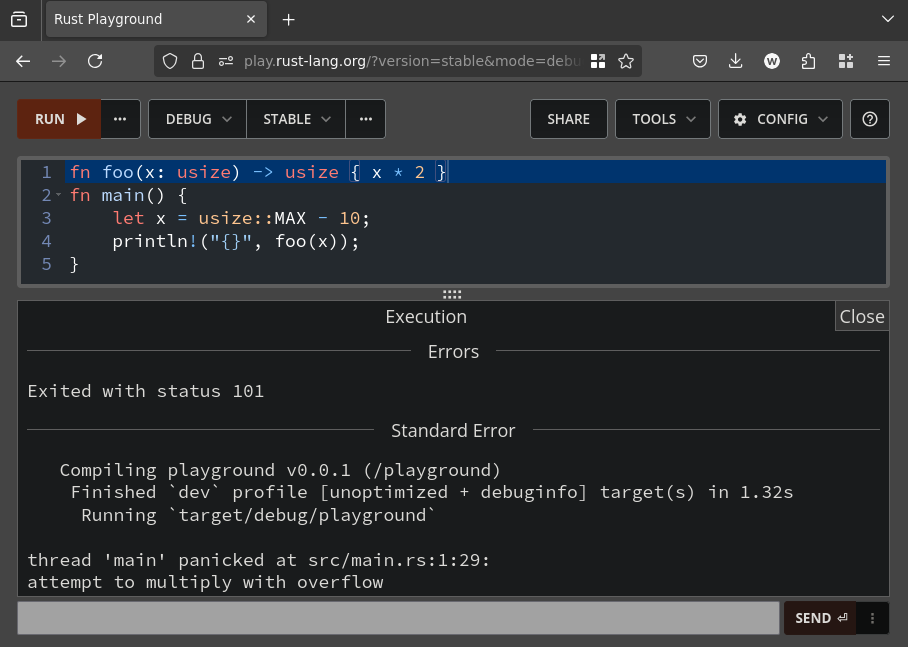
\includegraphics[height=0.9\textheight]{../overflow-int/rust-oflow-trap}
\end{frame}

\begin{frame}[fragile]{in Rust (2)}
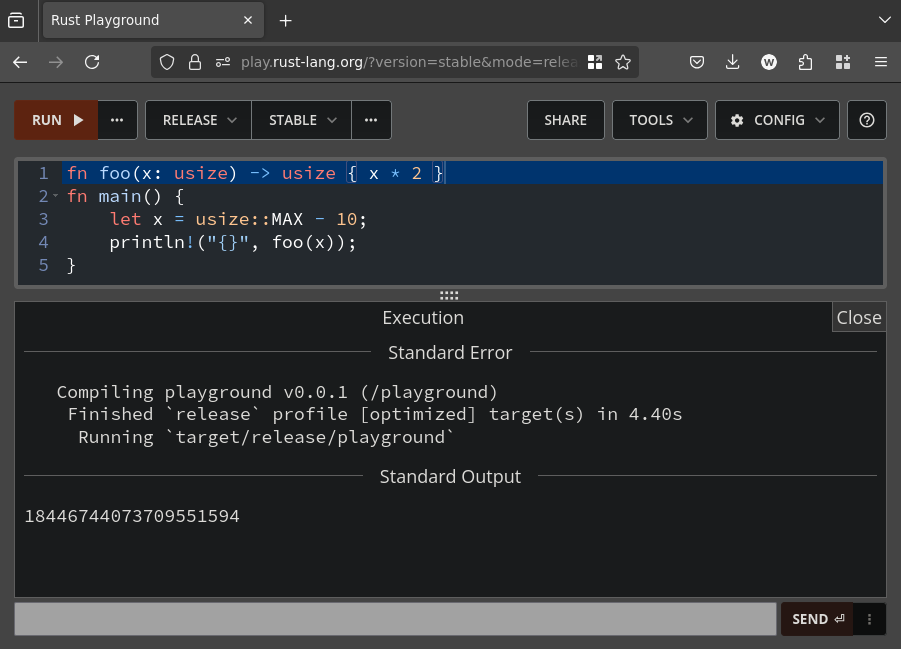
\includegraphics[height=0.9\textheight]{../overflow-int/rust-oflow-notrap}
\end{frame}

\begin{frame}[fragile]{in Rust (3)}
\begin{Verbatim}[fontsize=\fontsize{11}{12}]
let x = usize::MAX - 10; let y = 10usize;
println!("{} {}", x.saturating_mul(2), y.saturating_mul(2));
// 18446744073709551615 20
    // 18446744073709551615==usize::MAX
println!("{:?} {:?}", x.checked_mul(2), y.checked_mul(2));
// None Some(30)
println!("{} {}", x.wrapping_mul(2), y.wrapping_mul(2));
// 18446744073709551594 20
    // 18446744073709551594==usize::MAX-21
\end{Verbatim}
\end{frame}


\begin{frame}{compiler support to avoid?}
    \begin{itemize}
    \item GCC/Clang options:
        \begin{itemize}
        \item -fsanitize=undefined
        \item -ftrapv
        \end{itemize}
    \item better programming language design:
        \begin{itemize}
        \item Rust, \ldots
        \end{itemize}
    \end{itemize}
\end{frame}

% FIXME: examples of -fsanitize=undefined, -ftrapv
% FIXME: wrapping behavior in C for usnignedj
% FIXME: example in Rust + other int operators

\begin{frame}{overflow, C and undefined behavior}
\end{frame}
